\documentclass[a4paper,12pt]{article}

\usepackage{graphicx}
\usepackage[brazilian]{babel}
\usepackage[utf8]{inputenc}
\usepackage{fancyhdr}
\usepackage{hyperref}

\hypersetup{bookmarks=true, unicode=true, pdftoolbar=true, pdfmenubar=true, pdffitwindow=true}

\pagestyle{fancy}
\renewcommand{\headrulewidth}{0.0pt}
\renewcommand{\footrulewidth}{0.0pt}
\fancyhead{}
\fancyhead[C]{versão 0.15}

\def\cms{\emph{CMS}}
\def\rss{\emph{RSS}}
\def\plugin{\emph{plugin}}
\def\queue{\emph{Queue}}
\def\url{\emph{URL}}

\begin{document}

\title{Software para integração de \emph{feeds} e sistemas de gerenciamento de conteúdo}
\author{Marcelo Toledo \and Rafael Castilho}
\date{\today}

\maketitle

\newpage
\section{Introdução}

\paragraph{}
Sistemas de gerenciamento de conteúdo (\cms{}), em particular os populares
\emph{blogs}, são ferramentas que permitem a publicação de conteúdo em um
endereço \emph{WEB}, e que exigem apenas o conhecimento do uso da
\emph{interface}.

\paragraph{}
Em geral, os \cms{}s permitem a visualização de itens de conteúdo publicado na
forma parametrizada \rss{} por meio de canais alimentadores (\emph{feeds}). Uma
das ferramentas mais utilizadas pelos \emph{blogueiros} é o agregador de
\rss{}, capaz de coletar e organizar o conteúdo de diversos canais
simultaneamente.

\paragraph{}
Em um \emph{blog}, além de conteúdo próprio, é comum a citação de conteúdo de
terceiros, realizado de forma "artesanal", através da cópia das informações
disponíveis na página \emph{WEB} ou no agregador e da colagem no editor de
publicação do \cms{}.

\paragraph{}
O objetivo do software a ser desenvolvido é disponibilizar um agregador de
canais que permita a publicação de itens de conteúdo no \cms{} do cliente de
forma ágil, padronizada, e com base em suas preferências.

\section{Especificação funcional}

\subsection{Cadastro de perfil de acesso}

\paragraph{}
Para ter acesso ao software, o cliente deve efetuar a autenticação de um perfil
de acesso a partir de um endereço de e-mail e senha cadastrados.

\subsubsection{Novo perfil}

\paragraph{}
O cadastro de um novo perfil de acesso é feito a partir do formulário de
autenticação, através da opção "não cadastrado", que quando acionada, passa a
exibir o formulário para um novo cadastro. 

\begin{center}
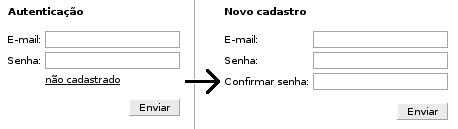
\includegraphics[scale=0.8]{authform.png}
\end{center}

\paragraph{}
O procedimento para criação de um novo perfil a partir do formulário para um
novo cadastro deve ser feito como segue:

\begin{enumerate}
\item Informar um endereço de e-mail, senha e confirmação de senha;
\item Se o endereço de e-mail não estiver cadastrado em um perfil de acesso, o
cliente deverá receber uma mensagem de e-mail contendo uma \url{} de
confirmação de cadastro;
\item Após a confirmação de cadastro, o cliente deverá reber uma mensagem de
e-mail contendo uma notificação de cadastro confirmado e instruções para o
primeiro acesso.
\item Se o endereço de e-mail informado já estiver cadastrado, o cliente deverá
receber uma mensagem de e-mail contendo uma notificação da existência do perfil
com instruções para acesso e alteração de senha (se necessário).
\end{enumerate}

\subsubsection{Atualização de perfil}

\paragraph{}
Após efetuar o acesso, o cliente poderá alterar suas informações de acesso e
preencher os seguintes dados pessoais:

\begin{itemize}
\item Nome;
\item País;
\item Região;
\item Cidade;
\item Distrito;
\item Endereço;
\item Código postal
\end{itemize}

Para alteração do endereço de e-mail, o cliente deverá efetuar o seguinte
procedimento:

\begin{enumerate}
\item Acionar o comando de alteração de endereço de e-mail, que enviará uma
mensagem ao endereço atual com instruções para alteração.
\item A mensagem deve conter uma \url{} que permite acesso ao formulário de
alteração de endereço de e-mail, onde o cliente deve informar o novo endereço.
\item Uma mensagem deve ser enviada ao antigo e novo endereços notificando a
alteração.
\end{enumerate}

\subsubsection{Recuperação de acesso}

\paragraph{}
O software deve permitir ao cliente recuperar o acesso quando não recordar sua
senha, através do seguinte procedimento:

\begin{enumerate}
\item Informar o endereço de e-mail do perfil de acesso;
\item Se o endereço de e-mail estiver cadastrado em um perfil de acesso, o
cliente receberá uma mensagem de e-mail com uma \url{} para o formulário de
alteração de senha;
\item O formulário de alteração de senha deve permitir ao cliente digitar uma
nova senha. Após a alteração, o software deverá enviar uma mensagem de e-mail
ao cliente com a notificação de alteração.
\item Se o endereço de e-mail informado não estiver associado a um perfil de
acesso, o cliente deverá receber uma mensagem de e-mail com a notificação da
não existência do perfil de acesso e instruções para a criação de um novo.
\end{enumerate}

\subsection{Cadastro de \cms{}}

\subsubsection{Novo \cms{}}

\paragraph{}
Após efetuar acesso, o cliente poderá realizar o cadastro de um novo \cms{}
através das seguintes etapas:

\begin{enumerate}
\item Informar a \url{} raiz do \cms{}. O software deverá detectar o tipo de
\cms{} (\emph{Wordpress}, \emph{Joomla}, \emph{Drupal}, etc.) a partir da
\url{} informada;
\item Se for possível a detecção do tipo de \cms{}, o software deverá verificar
a existência do gerenciador de publicações do \cms{} em um endereço padrão, de
acordo com o tipo de \cms{} e da \url{} raiz;
\item Se o gerenciador de publicações do \cms{} não estiver disponível no
endereço padrão, permitir que o cliente informe seu endereço através de uma
\url{}. O software deverá verificar se o endereço informado é válido como
gerenciador de publicações para o tipo de \cms{} escolhido;
\item Se a detecção do tipo de \cms{} não for bem sucedida, verificar a causa e
informar o erro mais provável (endereço ou página não encontrados, erro no
servidor, etc.);
\item Se o endereço estiver correto mas o tipo não for suportado, exibir
notificação ao cliente e informar os tipos suportados. Permitir também que o
cliente digite o tipo utilizado. Neste caso, o cadastro de \cms{} não poderá
ser efetivado;
\item Após a determinação correta do tipo de \cms{} e endereço do gerenciador
de publicações, solicitar ao cliente que informe o usuário e senha do
gerenciador. O software deverá verificar se o usuário e senha permitem
autenticação no gerenciador, caso contrário, notificar que o usuário e senha
não são válidos;
\item O software deve verificar de forma não invasiva (sem publicar conteúdo em
produção) se o acesso ao gerenciador de publicações possui permissão para
escrita de conteúdo (ex. \emph{drafts} do \emph{Wordpress}). Se não for
possível tal verificação, o software poderá solicitar ao cliente se deseja
realizar um teste de publicação em produção.
\end{enumerate}

\subsubsection{Tipo de \cms{}}

\paragraph{}
O tipo de \cms{} define qual software é utilizado pelo cliente. Os tipos
disponíveis serão adicionados ao software na forma de \emph{plugins}, e devem
implementar uma interface determinada pelo software.

% TODO: definir os métodos da interface de plugins

\paragraph{}
Um \emph{plugin} de \cms{} deve ser capaz de gerenciar as diferentes versões de
um tipo de \cms{}.

\subsubsection{Recursos}

\paragraph{}
O cliente poderá definir para cada \cms{} cadastrado, quais recursos serão
utilizados. Os recursos caracterizam o tipo de informação utilizada na
publicação de conteúdo em um \cms{}.

\paragraph{}
A disponibilidade de recursos depende do tipo de \cms{}. O software deve
estabelecer os recursos mínimos e obrigatórios e que devem ser implementados
para qualquer tipo, dos quais:

\begin{itemize}
\item Título;
\item Descrição;
\item Comentários;
\item Fonte (endereço de origem do conteúdo);
\end{itemize}

\paragraph{}
Outros recursos poderão ser utilizados conforme a disponibilidade, como por
exemplo:

\begin{itemize}
\item Categoria;
\item Data de publicação;
\item \emph{Tags};
\item etc.;
\end{itemize}

\paragraph{}
Os recursos que forem dependentes da entrada de informações pelo cliente (ex. Comentários, Categoria, etc.), só poderão ser utilizados através do método manual de publicação de conteúdo.

\subsubsection{Método de publicação}

\paragraph{}
O cliente poderá definir para cada \cms{} cadastrado a forma como este deverá
gerenciar a publicação dos itens de conteúdo disponíveis.

\paragraph{}
Por padrão, a publicação de conteúdo deve ser feita manualmente. No entanto é
possível automatizar este processo, a partir das seguintes configurações:

\begin{itemize}

% TODO: talvez aqui sejam duas coisas distintas: alimentacao/ordenacao de acordo com o queue, e frequencia, palavras-chave, com estrela (metodo de publicacao < este nome está legal?)

% \item Alimentação: Define a lista de canais a serem utilizados. Padrão: Todos
% os cadastrados;
% \item Ordenação: Define a ordem de publicação a partir da data de publicação,
% popularidade ou randômico. Padrão: Data de publicação;
\item Frequência: Define o intervalo de tempo entre as publicações (5min 15min,
30min, 1hora, 2hrs, 3hrs, 6hrs, 12hrs, 24hrs, etc.);
\item Palavras-chave: A escolha de itens é feita com base em uma ou mais
palavras-chave;
\item Com estrela: Somente itens de conteúdo marcados com estrela serão
utilizados para publicação;
\end{itemize}

\paragraph{}
Independentemente da configuração estabelecida para a publicação automática, a
opção manual deverá sempre estar disponível.


% \paragraph{}
% A popularidade pode ser medida através da quantidade de publicações feitas por
% outros clientees para um mesmo item.

%%% < TODO

\subsection{Cadastro de \rss{}}

\paragraph{}
O cadastro de canais \rss{} deverá ser particular a um \cms{} cadastrado.


\subsubsection{Novo \rss{}}

\paragraph{}
Para incluir um novo canal \rss{}, o cliente deve informar a \url{} do
alimentador ou um arquivo de importação \emph{OPML}.

\subsection{\emph{Dashboard}}

O \emph{dashboard} é a visualização padrão após a autenticação, composto por
painéis que permitem o gerenciamento das informações. 

\begin{center}
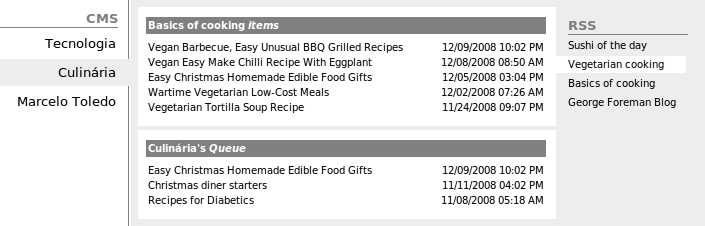
\includegraphics[scale=0.5]{dashboard.png}
\end{center}

\subsubsection{Painel de \cms{}}

O painel de \cms{} 

\subsubsection{Painel de \rss{}}

% TODO: A barra de canais \rss deve permitir ordenação através de drag'n'drop. A ordem do canal determina a importancia de um item de conteudo (sugestão do marcelo). Não seria melhor talvez colocar nota de 1-5 no canal e isto determinaria a importancia?

\paragraph{}
Durante a sessão de um perfil, o software deverá exibir a área de trabalho,
contendo painéis com a listagem de canais \rss{} e \cms{} cadastrados.

\paragraph{}
Em um painel central, serão exibidos os itens disponíveis de todos os canais
\rss{} cadastrados no perfil. Ao selecionar um canal, o painel deverá exibir
apenas os itens do canal selecionado.

\subsubsection{Área de \emph{Queue}}

\paragraph{}
O cliente poderá determinar a quantidade de itens de conteúdo que devem
aparecer no painel central, de acordo com as suas preferências.

\paragraph{}
A ordem de visualização dos itens é por padrão em ordem decrescente da data de
publicação, mas também poderá ser ordenado pela popularidade ou de forma
randômica.

\paragraph{}
Um item poderá ser marcado com uma estrela, permitindo que seja facilmente
encontrado posteriormente.

\paragraph{}
Um item de conteúdo poderá ser "arrastado" para um item do painel de \cms{}. Em
seguida, uma janela de publicação será exibida, onde o cliente deverá acionar o
botão "enviar" para publicar o conteúdo no \cms{}.

\subsubsection{Janela de publicação}

\paragraph{}
A janela de publicação deve conter o título e descrição do item de conteúdo,
além de um campo para adicionar comentários. A janela deve permitira a edição
dos valores iniciais.

\paragraph{}
Outros recursos podem estar disponíveis conforme o \cms{} utilizado.

\subsection{Gerenciador interno de conteúdo}

\paragraph{}
Os itens de conteúdo de um canal podem ser globais, ou seja, podem ser
compartilhados por todos os clientees do software, afim de eliminar redundância
desnecessária de dados.

\paragraph{}
Quando um novo canal é adicionado, o sistema se preocupa em obter os itens mais
recentes deste canal imediatamente.

\paragraph{}
Para um canal já existente, o sistema deverá executar em \emph{background} e
obter novos itens, com uma freqüência que depende da freqüencia de publicação
de conteúdo neste canal.



\appendix

\section{Notas}

\paragraph{}
Quando um tipo de \cms{} não for suportado, e o cliente informar o tipo de
\cms{} utilizado, o \emph{backend} poderá verificar se houve falha na detecção
e solicitar ajuste no desenvolvimento, e informar ao cliente sobre a resolução
do problema. Se o tipo não for suportado, informar ao cliente que o software
não é suportado. É possível também verificar quais são as tendências para
implementações de novos tipos.

\paragraph{}
O software deverá servir como guia para padronização da publicação de conteúdo
externo, com a virtude de previnir ao cliente problemas com \emph{copyright},
por exemplo.

\subsection{Segurança}

\paragraph{}
O software deve limitar a quantidade de mensagens de e-mail enviadas durante a
solicitação de um novo cadastro de perfil ou durante a recuperação de acesso a
um perfil de acesso, afim de evitar uso mal intencionado do envio de mensagens.

\paragraph{}
O software deve conter algum tipo de proteção para que as publicações em um
\cms{} não sejam feitas por seu próprio alimentador automaticamente e
indefinidamente (autófago).

\end{document}
